\begin{figure}[!htb]
    \centering
    \begin{subfigure}[b]{0.49\textwidth}
        \centering
        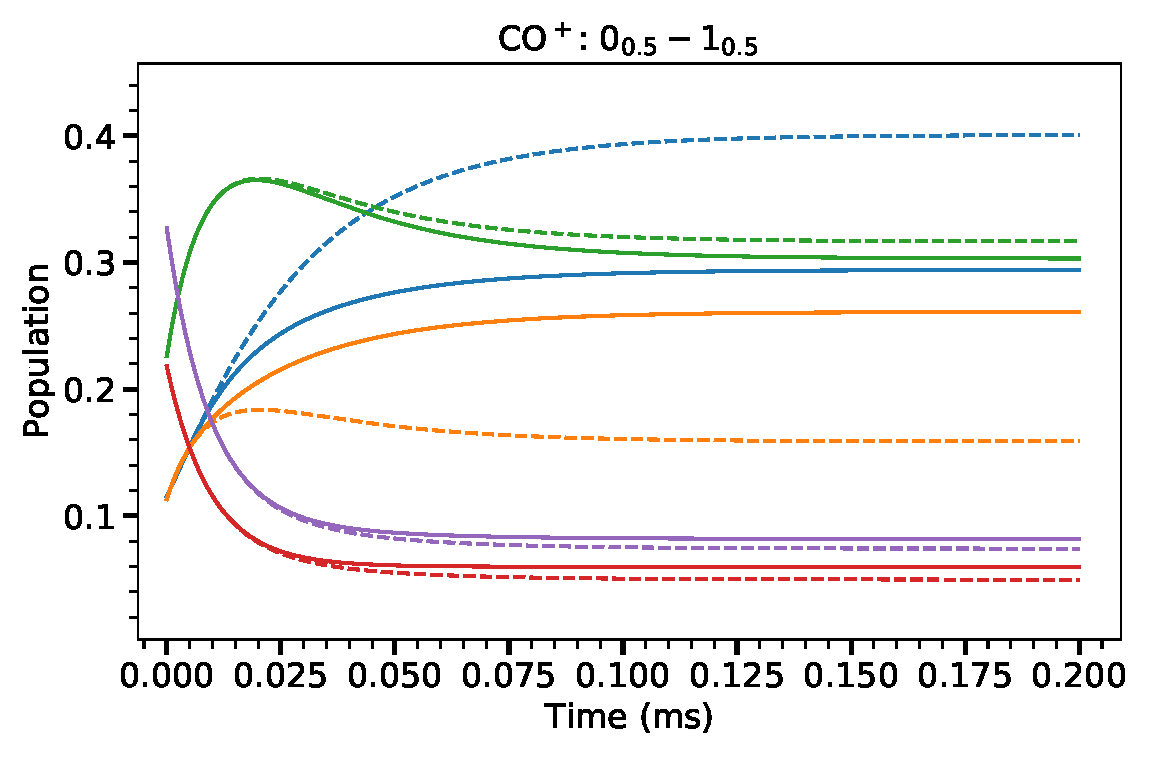
\includegraphics[width=1\textwidth]{chapters/CO+_ROSAA_paper/SI/CO^+_pop_ratio_0_0.5 - 1_0.5.pdf}
        \caption{}
    \end{subfigure}
    \hfill
    \begin{subfigure}[b]{0.49\textwidth}
        \centering
        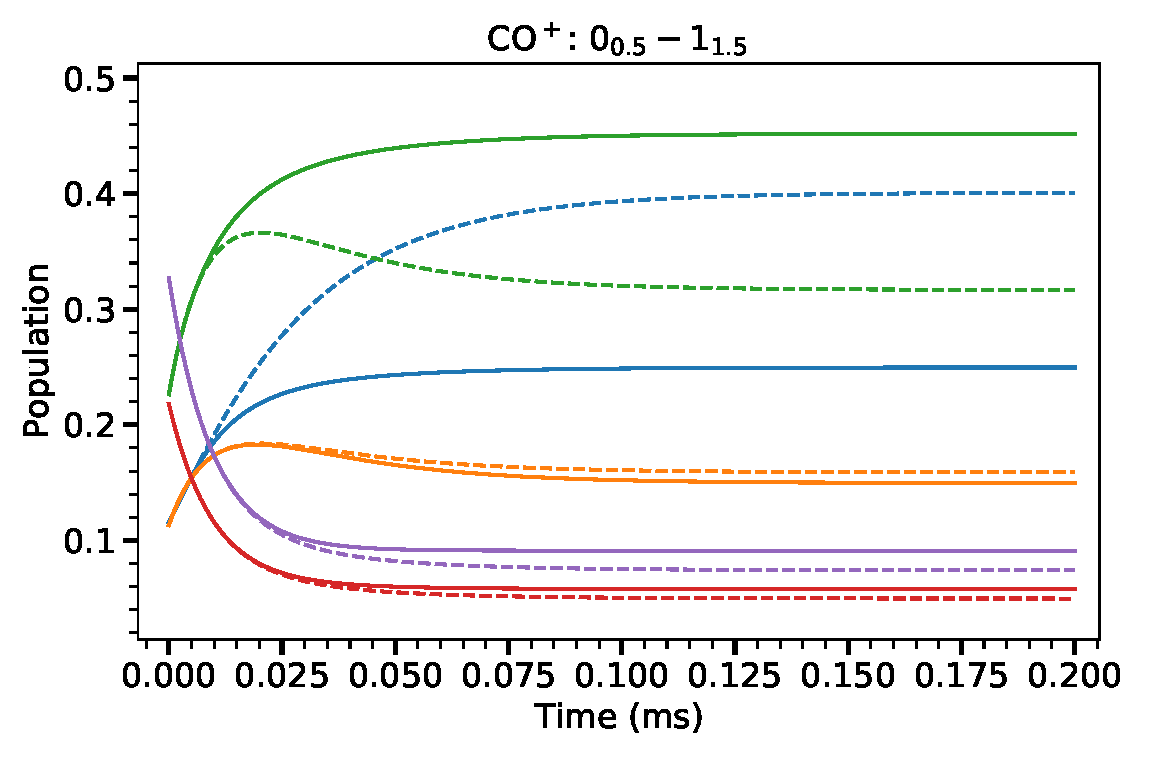
\includegraphics[width=1\textwidth]{chapters/CO+_ROSAA_paper/SI/CO^+_pop_ratio_0_0.5 - 1_1.5.pdf}
        \caption{}
    \end{subfigure}
    \hfill
    \begin{subfigure}[b]{0.49\textwidth}
        \centering
        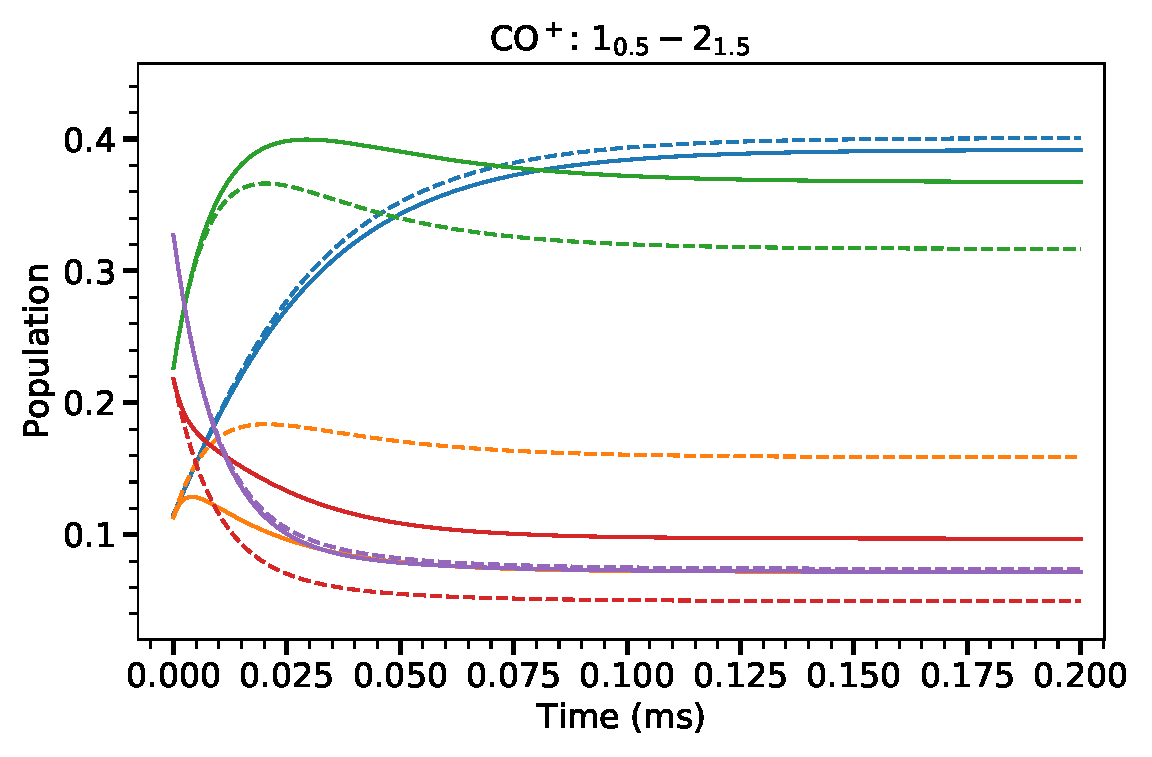
\includegraphics[width=1\textwidth]{chapters/CO+_ROSAA_paper/SI/CO^+_pop_ratio_1_0.5 - 2_1.5.pdf}
        \caption{}
    \end{subfigure}
    \hfill
    \begin{subfigure}[b]{0.49\textwidth}
        \centering
        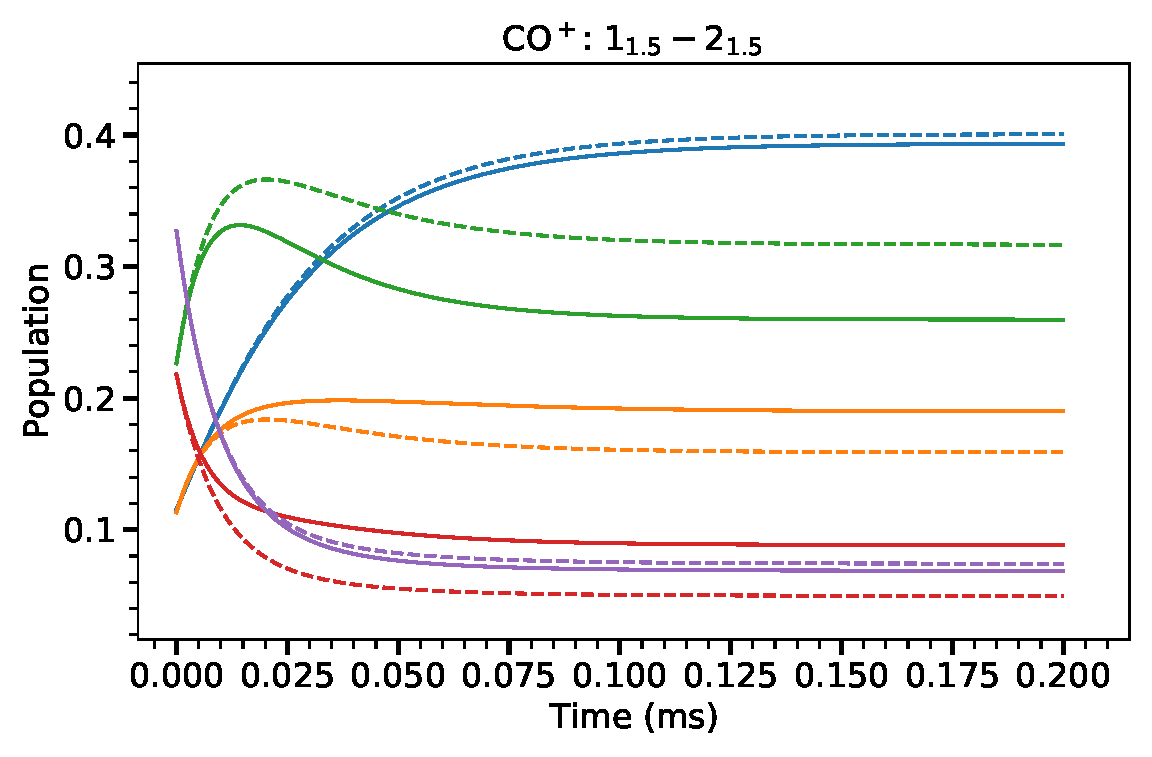
\includegraphics[width=1\textwidth]{chapters/CO+_ROSAA_paper/SI/CO^+_pop_ratio_1_1.5 - 2_1.5.pdf}
        \caption{}
    \end{subfigure}
    \caption{Numerical simulations of the rotational state population distribution of $N_J$ states with (solid line) and without (dashed line) radiation upon excitation of the transitions indicated in the title of each figure. The color code represents $N_J$ states as follows: \textcolor{blue}{\co($0_{0.5}$)}, \textcolor{orange}{\co($1_{0.5}$)}, \textcolor{green}{\co($1_{1.5}$)}, \textcolor{red}{\co($2_{1.5}$)} and  \textcolor{purple}{\co($2_{2.5}$)}. At t=0, the initial population is given by the  Boltzmann distribution at T=300 K which undergoes collisional cooling to reach collisional temperature T=$6(1)$K. The collisional rates are computed from collisional rate constants and He number density [He]$\sim 4\cdot10^{14}$~cm$^{-3}$. The radiative rates (Einstein B  coefficients for stimulated emission and absorption) are derived from Einstein A coefficients for spontaneous emission (PGOPHER simulation) with radiation power for (a) \& (b) 25$\mu W$ and (c) \& (d) 20$\mu W$.}
\end{figure}

\begin{figure}[!htb]
    \centering
    \begin{subfigure}[b]{0.49\textwidth}
        \centering
        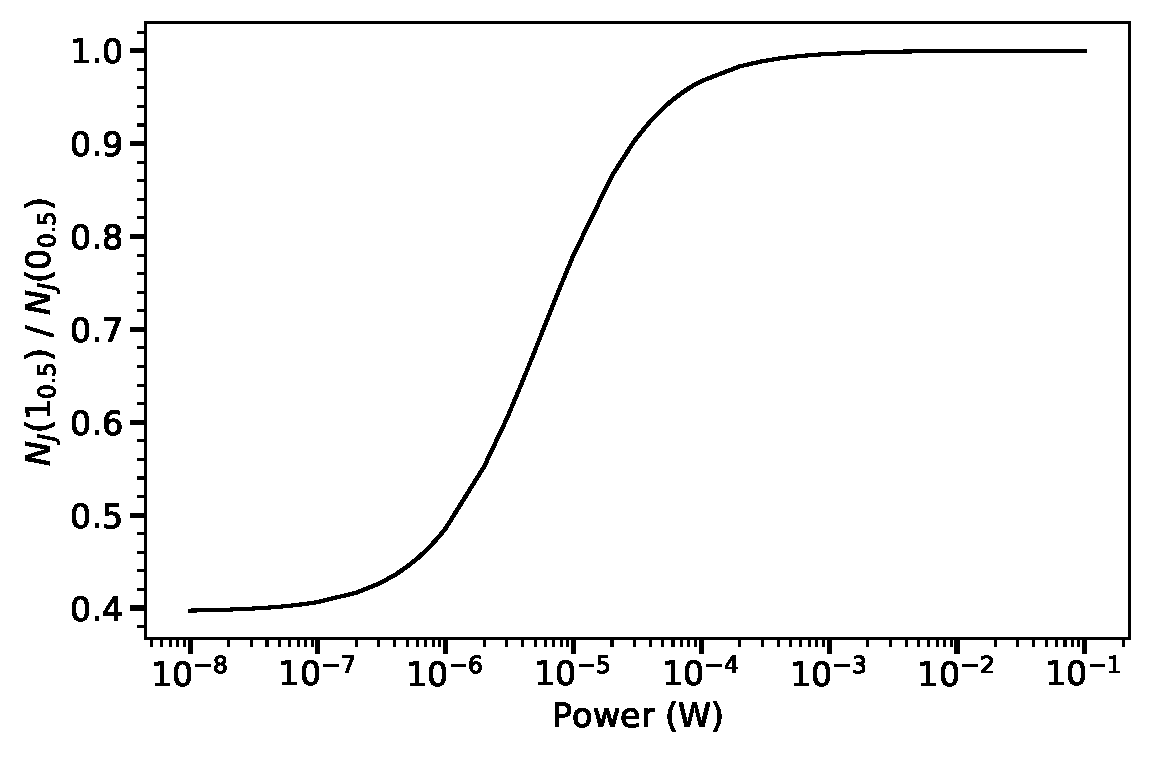
\includegraphics[width=1\textwidth]{chapters/CO+_ROSAA_paper/SI/functionOfpower_CO^+_0_0.5 - 1_0.5_4.e+14.pdf}
    \end{subfigure}
    \hfill
    \begin{subfigure}[b]{0.49\textwidth}
        \centering
        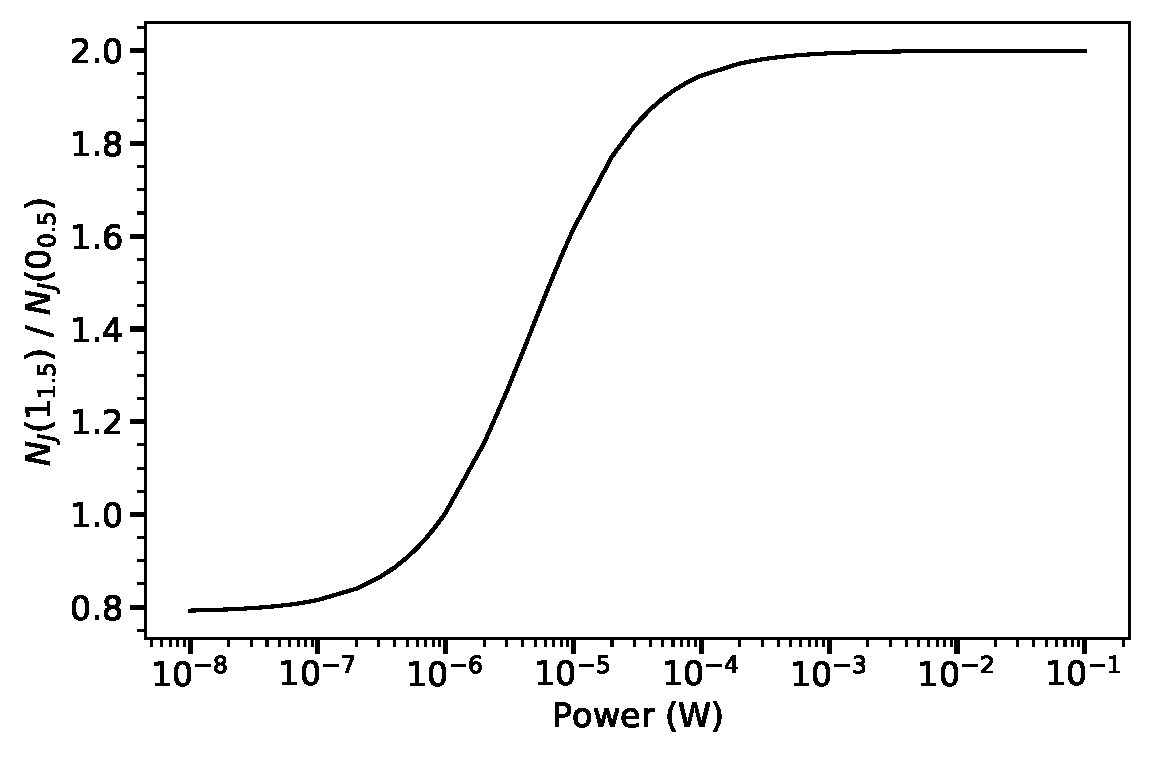
\includegraphics[width=1\textwidth]{chapters/CO+_ROSAA_paper/SI/functionOfpower_CO^+_0_0.5 - 1_1.5_4.e+14.pdf}
    \end{subfigure}
    \hfill
    \begin{subfigure}[b]{0.49\textwidth}
        \centering
        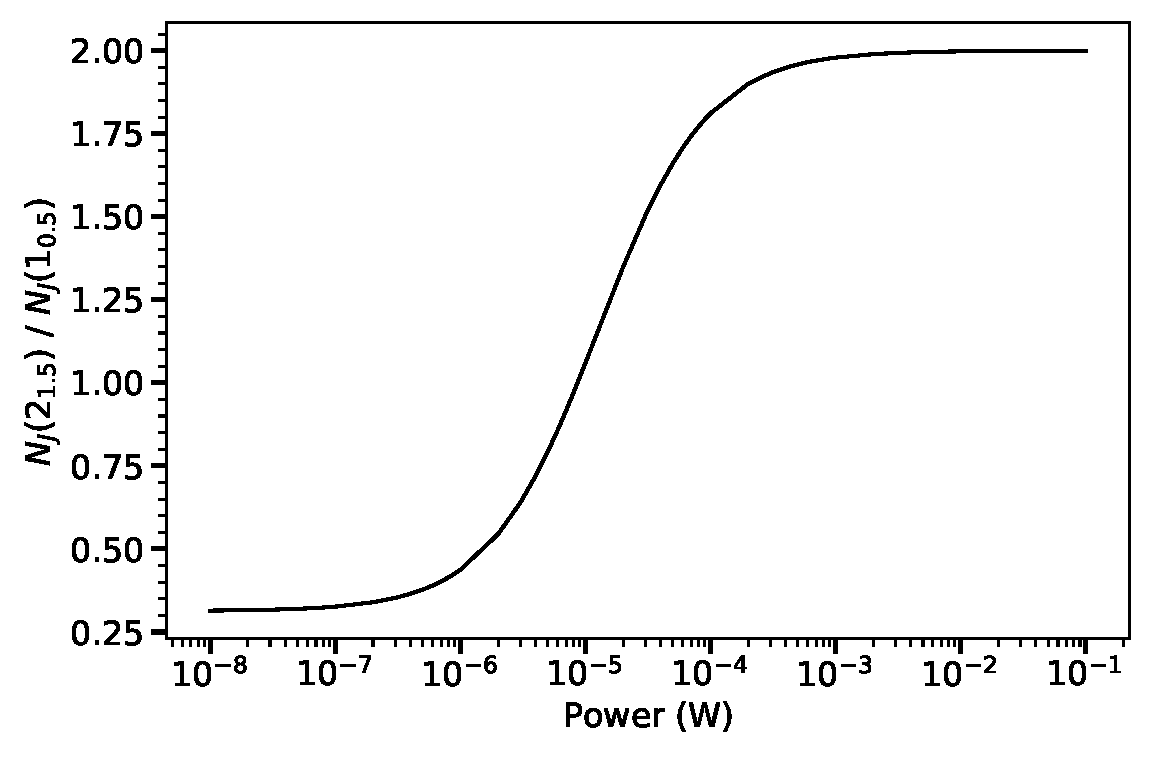
\includegraphics[width=1\textwidth]{chapters/CO+_ROSAA_paper/SI/functionOfpower_CO^+_1_0.5 - 2_1.5_4.e+14.pdf}
    \end{subfigure}
    \hfill
    \begin{subfigure}[b]{0.49\textwidth}
        \centering
        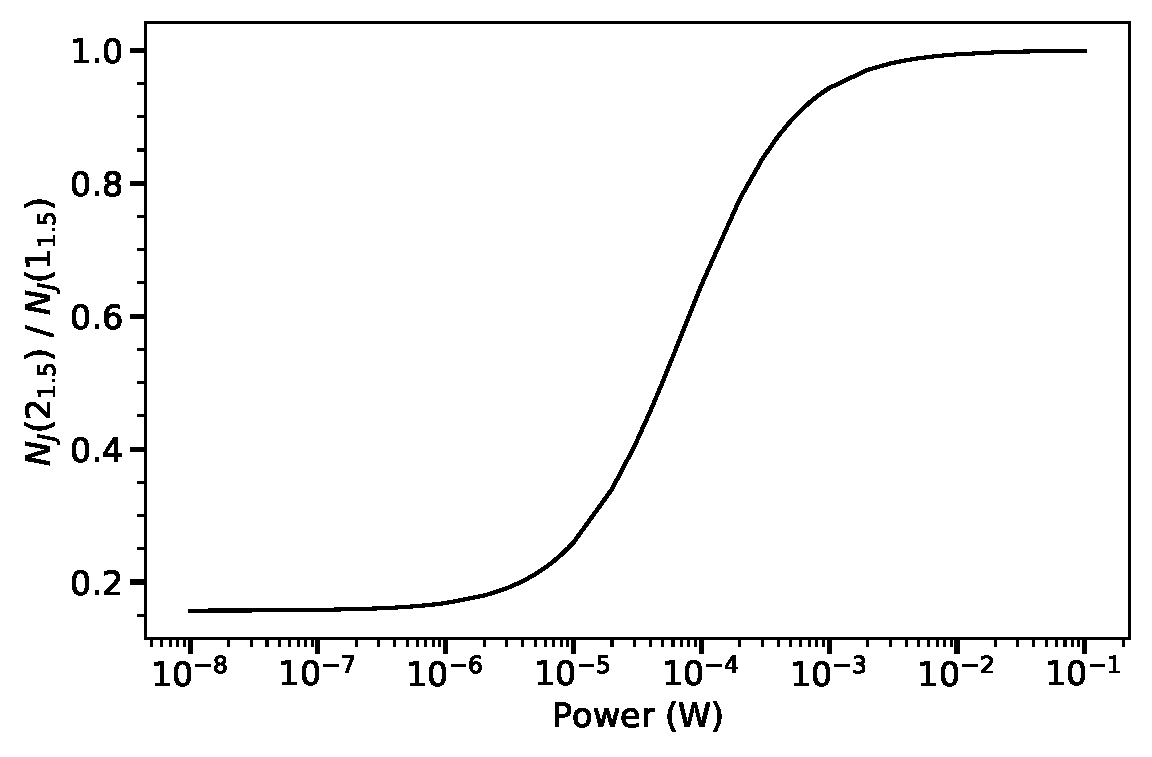
\includegraphics[width=1\textwidth]{chapters/CO+_ROSAA_paper/SI/functionOfpower_CO^+_1_1.5 - 2_1.5_4.e+14.pdf}
    \end{subfigure}
    \caption{Simulated population ratio ($N_J$: up/down) of CO$^+$ fine-structure transitions as a function of continuous excitation power on the respective transition after storing for 600ms in the trap with a constant He number density of [He]$\sim4\cdot$10$^{14}$~cm$^{-3}$.}
    \label{fig:SI:CO+:power}
\end{figure}

\begin{figure}
    \centering
    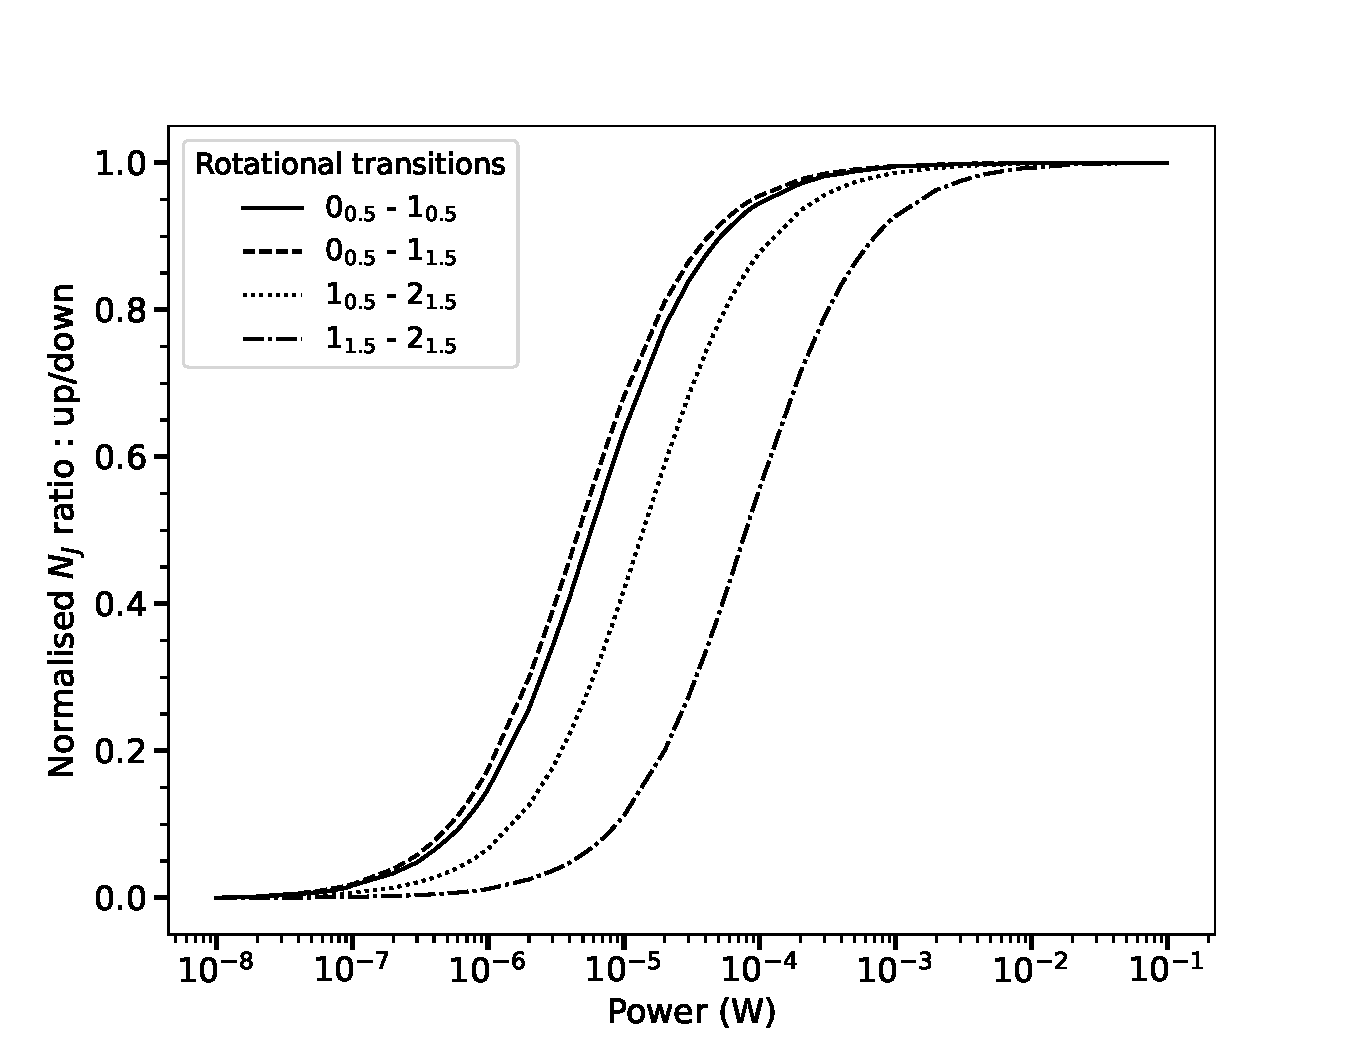
\includegraphics[width=1\textwidth]{chapters/CO+_ROSAA_paper/SI/compareTransitions.pdf}
    \caption{Comparison of the normalized simulated population ratio ($N_J$: up/down) of the respective CO$^+$ fine-structure transitions as a function of continuous excitation power on the respective transition after storing for 600ms in a trap with a constant He number density of [He]$\sim4\cdot$10$^{14}$~cm$^{-3}$. Transitions with higher transition strength reach saturation at lower excitation power.}
    \label{fig:SI:CO+:power-norm}
\end{figure}